\input{head-vertiefung.inc}
\usepackage{tikz-3dplot}
% Präambelbefehle für die Präsentation
\title[TET Vertiefung: Spiegelungsmethode -- Beispiele]{Spiegelungsmethode -- Beispiele}

\begin{document}
% 
% Frontmatter 
% 
%%%%%%%%%%%%%%%%%%%%%%%%%%%%%%%%%%%%%%%%%%%%%%%%%%%%%%%%%%%%%%%%%%%%%%%%%%%%%%%%%%%%%%%%%%%%%%%%%%%%%%%%%%%%%%%%%%%%%%%%%%%%% 

%% inserts the title page and the table of contents
\maketitle

% 
% Content 
% 
%%%%%%%%%%%%%%%%%%%%%%%%%%%%%%%%%%%%%%%%%%%%%%%%%%%%%%%%%%%%%%%%%%%%%%%%%%%%%%%%%%%%%%%%%%%%%%%%%%%%%%%%%%%%%%%%%%%%%%%%%%%%% 
\section{Spiegelung - Beispiele}


\begin{frame}
  \frametitle{Spiegelung an einer Ebene}
  \begin{columns}
    \begin{column}{.3\textwidth}
     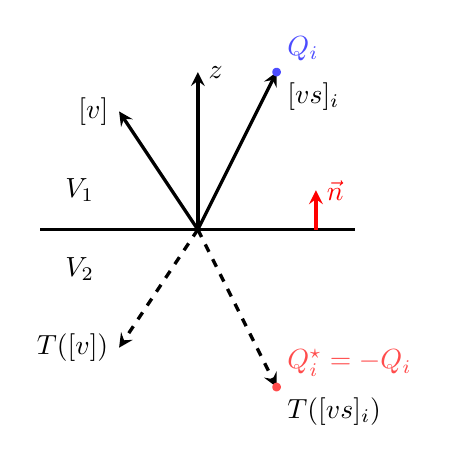
\begin{tikzpicture}[line width = 1.2pt, line join=round,>=stealth]
       \coordinate (O) at (0,0);
       \coordinate (a) at (-2,0);
       \coordinate (b) at (2,0);
       \draw (a) -- (b);
       \draw[color=red, -stealth] (1.5,0) -- (1.5,.5) node[right] {$\vec{n}$}; 
       \draw[ -stealth] (O) -- (0,2) node[right] {$z$}; 
       \draw[ -stealth] (O) -- (-1,1.5) node[left] {$\Ortsr[v]$}; 
       \draw[ dashed, -stealth] (O) -- (-1,-1.5) node[left] {$T(\Ortsr[v])$}; 
       \draw[ -stealth] (O) -- (1,2) node[below right] {$\Ortsr[vs]_i$};
       \filldraw [color=blue!70] (1,2) circle (1pt) node[above right] {$Q_i$}; 
       \draw[ dashed, -stealth] (O) -- (1,-2) node[below right] {$T(\Ortsr[vs]_i)$};
       \filldraw [color=red!70] (1,-2) circle (1pt) node[above right] {$Q_i^\star=-Q_i$}; 
\draw(-1.5,0.5) node {$V_1$}; 
\draw(-1.5,-0.5) node {$V_2$}; 

\end{tikzpicture}
\end{column}
\begin{column}{.65\textwidth}
  \begin{itemize}[<+->]
  \item Abbildung $T$ intuitiv klar
    \begin{align*}
      T:\; &\mathbb{R}^3 \to \mathbb{R}^3: \; \Ortsr[v] \to T(\Ortsr[v]) \nonumber\\
      \Aboxed{&T(\Ortsr[v]) = \Ortsr[v] - 2 \vec{n} (\vec{n}\cdot \Ortsr[v])}
    \end{align*}
  \item Funktion $\lambda$ intuitiv klar:
    \begin{align*}
      \lambda:\; &V_1\cup O(V_2) \to \mathbb{R}: \Ortsr[vs] \to \lambda(\Ortsr[vs])\nonumber\\
      \Aboxed{&\lambda(\Ortsr[vs]) = 1}
    \end{align*}
    \item Anforderungen offensichtlich erfüllt: Bildladungen in $V_2$, $O(V_2)$ wird auf sich selbst abgebildet, $\lambda(\Ortsr[vs]) = 1$ für $\Ortsr[vs] \in O(V_2)$ 
    \end{itemize}
  \end{column}
\end{columns}
\pause
\begin{itemize}
\item Für $\SkalarPot = 0$ auf $O(V_2)$: Umwälzen von Quellpunkt zum Aufpunkt:
  \begin{equation*}
    \lambda(\Ortsr[vs]_i) G(\Ortsr[v],T(\Ortsr[vs]_i)) \stackrel{!}{=}  \lambda(\Ortsr[v]) G(T(\Ortsr[v]),\Ortsr[vs]_i) \text{ erfüllt, weil G nur vom Abstand abhängt}
    \end{equation*}
  \end{itemize}
\end{frame}

\begin{frame}
\frametitle{Umwälzung formal nachrechnen}

\begin{itemize}[<+->]
\item Nachrechnen, dass $T(T(\Ortsr[v])) = \Ortsr[v]$ ist:
  \begin{align*}
    T(T(\Ortsr[v])) &= T(\Ortsr[v] - 2 \vec{n} (\vec{n}\cdot \Ortsr[v]))\\
    & = \Ortsr[v] - 2 \vec{n} (\vec{n}\cdot \Ortsr[v]) - 2 \vec{n} (\vec{n}\cdot \left\{ \Ortsr[v] - 2 (\vec{n}\cdot \Ortsr[v]) \vec{n}  \right\} )  \\ 
    & = \Ortsr[v] - 2 \vec{n} (\vec{n}\cdot \Ortsr[v]) - 2 \vec{n} (\vec{n}\cdot \Ortsr[v] - 2 \vec{n}\cdot \Ortsr[v])\\   
                         & = \Ortsr[v] - 2 \vec{n} (\vec{n}\cdot \Ortsr[v]) - 2 \vec{n} (- \vec{n}\cdot \Ortsr[v]) = \Ortsr[v]
  \end{align*}
\item Betrag von $\left|T(\Ortsr[v])\right|$:
  \begin{equation*}
    \left|T(\Ortsr[v])\right| = \left| \Ortsr[v] - 2 (\vec{n}\cdot \Ortsr[v]) \vec{n} \right| = \left| \Ortsr[v] \right| \text{ weil nur Vorzeichen der Normalkomponente geändert}
    \end{equation*}
  \item Umwälzung nachrechnen:
    \begin{align*}
      G(\Ortsr[v], T(\Ortsr[vs])) &= \frac{1}{4\pi\varepsilon_1} \frac{1}{\left|\Ortsr[v] -  T(\Ortsr[vs]) \right|} = \frac{1}{4\pi\varepsilon_1} \frac{1}{\left|T(T(\Ortsr[v])) - T(\Ortsr[vs]) \right|} \text{ wegen } T(T(\Ortsr[v])) = \Ortsr[v]\\
      &= \frac{1}{4\pi\varepsilon_1} \frac{1}{\left|T( T(\Ortsr[v]) - \Ortsr[vs] )\right|} \text{ weil } T \text{ linear ist}\\
                                          &= \frac{1}{4\pi\varepsilon_1} \frac{1}{\left| T(\Ortsr[v]) - \Ortsr[vs] \right|} \text{ weil } \left|T(\Ortsr[v])\right| = \left| \Ortsr[v] \right| \\
                                            &= G(T(\Ortsr[v]), \Ortsr[vs])
    \end{align*}
   
  \end{itemize}


\end{frame}


\begin{frame}
  \frametitle{Spiegelung - Problemangepasste Greensche Funktion}

\begin{itemize}[<+->]
\item Problemangepasste Greensche-Funktion:
      \begin{align*}
         G^\star(\Ortsr[v],\Ortsr[vs]_i) & = G(\Ortsr[v],\Ortsr[vs]_i) -\lambda(\Ortsr[v]) G(T(\Ortsr[v]),\Ortsr[vs]_i)\\
         & = G(\Ortsr[v],\Ortsr[vs]_i) -\lambda(\Ortsr[vs]_i) G(\Ortsr[v],  T(\Ortsr[vs]_i))
      \end{align*}

    \item Mit $\lambda(\Ortsr[vs]) = 1$ und $T(\Ortsr[vs]) = \Ortsr[vs] - 2  \vec{n}  (\vec{n}\cdot \Ortsr[vs])$ folgt:
      \begin{equation*}
        G^\star(\Ortsr[v],\Ortsr[vs]) = \frac{1}{4\pi\varepsilon_1}  \left(  \frac{1}{\left|\Ortsr[v] -  \Ortsr[vs] \right|}  - \frac{1}{\left|\Ortsr[v] -  \left[ \Ortsr[vs] - 2 \vec{n} (\vec{n}\cdot \Ortsr[vs]) \right] \right|}\right)
      \end{equation*}
    \item Mit Hilfe der problemangepassten Greenschen Funktion kann das \alert{Diricletsche Randwertproblem} in $V_1 \cup O(V_2)$ als \alert{Freiraumproblem} gelöst werden. Die Randwerte (hier: Skalarpotential ist Null auf dem Rand) werden automatisch erfüllt.
    \item Das so gefundene Potential ist \alert{keine Lösung} in $V_2 \setminus O(V_2)$.
    \item Berechnung der influenzierten Oberflächenladungsdichte aus der (Un-)Stetigkeitsbedingung der Normalkomponente der Dielektrischen Verschiebung ($\to$ \texttt{TET-Elektrostatik-V-Spiegelungsmethode})
      \item Gesamtanordnung ist \alert{ungeladen} $\to$ kein Monopolterm
    \end{itemize}
  
\end{frame}

\begin{frame}
  \frametitle{Spiegelung an der Kante, $90^o$}

  \begin{columns}
    \begin{column}{.5\textwidth}
      \includegraphics[width=1.3\columnwidth]{Bildladung-36-45-60-72-90.png}
      \end{column}
      \begin{column}{.45\textwidth}
        \begin{itemize}[<+->]
        \item Kante durch zwei Ebenen $\vec{n}_1$ und $\vec{n}_2$
        \item Spiegelbilder der Spiegelladungen
        \item Spiegelladungen verboten in $V_1$
          \item Interessant: ganzzahlige Teile von $360^o$
          \end{itemize}
      \end{column}
    \end{columns}
    \pause
    Problemangepasste Greensche-Funktion:
    \begin{align*}
      G^\star(\Ortsr[v], \Ortsr[vs])  =\quad & G (\Ortsr[v], \Ortsr[vs]) & \text{Greensche-Funktion des Freiraums} \\
      & - G (\Ortsr[v], T_{\vec{n}_1}(\Ortsr[vs])) & \text{Spiegelung an Ebene } \vec{n}_1\\ 
                                               & - G (\Ortsr[v], T_{\vec{n}_2}(\Ortsr[vs])) & \text{Spiegelung an Ebene } \vec{n}_2\\
     & \underbrace{+}_{(-)( -)}  G (\Ortsr[v], T_{\vec{n}_2}(T_{\vec{n}_1}(\Ortsr[vs]))) & \text{Spiegelung der Spiegelung}
  \end{align*}
\end{frame}


\begin{frame}
  \frametitle{Spiegelung an der Kante (andere Winkel)}
  \begin{itemize}[<+->]
  \item Interaktive Analyse mit \alert{Geogebra Geometrie}\\
    Webseite: \url{https://www.geogebra.org}\\
    Online-Version: \url{https://www.geogebra.org/geometry}
    \item Datei \texttt{Bildladung-36-45-60-72-90.ggb} im OER-Ordner der Professur
  \end{itemize}
\end{frame}


\begin{frame}
  \frametitle{Spiegelung an der (geerdeten) Kugel}
  \begin{columns}
    \begin{column}{.35\textwidth}
      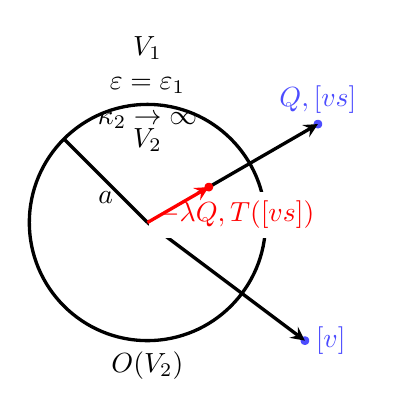
\begin{tikzpicture}[line width = 1.2pt, line join=round,>=stealth]
        \filldraw [color=blue!70] (30:2.5) circle (1pt) node[above] {$Q, \Ortsr[vs]$}; 
        \filldraw [color=blue!70] (2,-1.5) circle (1pt) node[right] {$\Ortsr[v]$}; 
        \draw [-stealth] (0,0) -- (30:2.5); 
        \draw [-stealth] (0,0) -- (2,-1.5); 
        \draw (0,0) circle (1.5);
        \draw (0,0) -- (135:1.5);
        \draw (135:0.75 ) node[below] {$a$};
        
        \draw (0,-1.5) node [below] {$O(V_2)$};
        \draw(0,1.05) node {$V_2$};
        \draw(0,1.3) node{$\kappa_2 \to \infty$};
        \draw(0,2.0) node[align=center] {$V_1$\\$\varepsilon=\varepsilon_1$}; 
       \draw [color=red] (20:1.2) node[below, fill=white] {$-\lambda Q, T(\Ortsr[vs])$}; 

       \draw [-stealth,color=red] (0,0) -- (30:0.9); 
       \filldraw [color=red] (30:0.9) circle (1pt);
      \end{tikzpicture}
      \end{column}
      \begin{column}{.5\textwidth}
        \begin{itemize}[<+->]
        \item Versuche die \alert{Kelvin-Transformation}:
          \begin{align*}
            T & :  \mathbb{R}^3 \to \mathbb{R}^3 : \Ortsr[vs] \to T(\Ortsr[vs]) = \frac{a^2}{\left| \Ortsr[vs]\right|^2} \Ortsr[vs] = a \frac{a}{\Ortsr[s]} \vu{\Ortsr[s]}\\
            \lambda & :  \mathbb{R}^3 \to \mathbb{R} : \Ortsr[vs] \to \lambda(\Ortsr[vs]) = \frac{a}{\left| \Ortsr[vs]\right|}  
          \end{align*}
        \item Für $\Ortsr[vs] \in O(V_2)$: $T(\Ortsr[vs]) = \Ortsr[vs]$
        \item $T(T(\Ortsr[vs])) = T(a \frac{a}{\Ortsr[vs]} \vu{\Ortsr[vs]}) =  a \frac{a}{a \frac{a}{\Ortsr[vs]}} \vu{\Ortsr[vs]} = \Ortsr[vs]$
        \item Regel der \alert{reziproken Radien}:
          \begin{equation*}
            \boxed{\left| \Ortsr[vs] \right| \left| T(\Ortsr[vs]) \right| = a^2}
            \end{equation*}
          \end{itemize}
        \end{column}
      \end{columns}
      \begin{itemize}[<+->]
        \item Die grundlegenden Bedingungen an die Transformation sind erfüllt. 
        \item Hinreichende Bedingung für $\SkalarPot = 0$ auf $O(V_2)$: Umwälzung von Quellpunkt und Aufpunkt
        \end{itemize}
\end{frame}

\begin{frame}
  \frametitle{Kugel: Umwälzung von Quellpunkt und Aufpunkt}
  \begin{itemize}[<+->]
  \item Zu zeigen:
    \(
      \lambda(\Ortsr[vs]) G(\Ortsr[v], T(\Ortsr[vs])) \stackrel{!}{=} \lambda(\Ortsr[v]) G(T(\Ortsr[v]), \Ortsr[vs]) 
    \)
  \item Zunächst:
    \begin{align*}
      \left| T(\Ortsr[v]) - \Ortsr[vs]  \right|^2 & = \left| \frac{a^2}{\left| \Ortsr[v]\right|^2} \Ortsr[v] - \Ortsr[vs] \right|^2 = \frac{a^4}{\left| \Ortsr[v]\right|^2} - \frac{2a^2}{\left| \Ortsr[v]\right|^2} \Ortsr[v] \cdot \Ortsr[vs] + \left| \Ortsr[vs]\right|^2 \\
                                                              & = \frac{\left| \Ortsr[vs]\right|^2}{\left| \Ortsr[v]\right|^2} \left[  \frac{a^4}{\left| \Ortsr[vs]\right|^2} - \frac{2a^2}{\left| \Ortsr[vs]\right|^2} \Ortsr[v] \cdot \Ortsr[vs] + \left| \Ortsr[v]\right|^2 \right] = \frac{\left| \Ortsr[vs]\right|^2}{\left| \Ortsr[v]\right|^2} \left| \Ortsr[v] - \frac{a^2}{\left| \Ortsr[vs]\right|^2} \Ortsr[vs]\right|^2\\
      & = \frac{\left| \Ortsr[vs]\right|^2}{\left| \Ortsr[v]\right|^2} \left| \Ortsr[v]   - T(\Ortsr[vs]) \right|^2
    \end{align*}
  \item Damit:
    \begin{align*}
      \lambda(\Ortsr[vs]) G(\Ortsr[v], T(\Ortsr[vs])) &= \frac{a}{\left| \Ortsr[vs]\right|} \frac{1}{4\pi\varepsilon_1}\frac{1}{\left| \Ortsr[v]   - T(\Ortsr[vs]) \right|} = \frac{a}{\left| \Ortsr[vs]\right|} \frac{1}{4\pi\varepsilon_1} \frac{\left| \Ortsr[vs]\right|}{\left| \Ortsr[v]\right|} \frac{1}{\left|  T(\Ortsr[v]) - \Ortsr[vs] \right|} \\
      &= \frac{a}{\left| \Ortsr[v]\right|} \frac{1}{4\pi\varepsilon_1} \frac{\left| \Ortsr[vs]\right|}{\left| \Ortsr[vs]\right|} \frac{1}{\left|  T(\Ortsr[v]) - \Ortsr[vs] \right|} = \lambda(\Ortsr[v]) G(T(\Ortsr[v]), \Ortsr[vs]) 
    \end{align*}
    \item Problemangepasste Greensche Funktion: $G^\star(\Ortsr[v], \Ortsr[vs]) = G(\Ortsr[v], \Ortsr[vs]) - \lambda(\Ortsr[vs]) G(\Ortsr[v], T(\Ortsr[vs])) $
    \end{itemize}
  \end{frame}

  \begin{frame}
    \frametitle{Isolierte Kugel -- Greensche-Funktion}
    \begin{itemize}[<+->]
    \item Bisher: \alert{geerdete Kugel} $\to$ beim Einbringen der Punktladung ändert sich die Ladung der Kugel durch elektrostatische Influenz.
    \item Kann man auch eine \alert{isolierte Kugel} behandeln?
    \item Bei der isolierten Kugel bleibt die Gesamtladung der Kugel beim Einbringen der Punktladung unverändert. Z.B. vorher Null $\to$ nachher Null.
    \item Die Bildladung $Q^\star = -\lambda(\Ortsr[vs]) Q$ verändert aber die Ladung im Volumen $V_2$
    \item Für eine (zusätzliche) Ladung im Zentrum der Kugel ist die Kugeloberfläche eine \alert{Äquipotentialfläche} $\to$ Potentialänderung nur um Konstante
    \item Größe der Ladung: $-Q^\star$
    \item Problemangepasste Greensche Funktion:
      \begin{align*}
        G^\star(\Ortsr[v], \Ortsr[vs]) & =  G(\Ortsr[v], \Ortsr[vs]) - \lambda(\Ortsr[vs]) G(\Ortsr[v], T(\Ortsr[vs])) + \lambda(\Ortsr[vs]) G(\Ortsr[v], \vec{0}) \\
& = G(\Ortsr[v], \Ortsr[vs]) - \frac{a}{\abs{\Ortsr[vs]}} \left( G\left(\Ortsr[v], \frac{a^2}{\abs{\Ortsr[vs]}^2} \Ortsr[vs]\right) - G(\Ortsr[v], \vec{0}) \right) \\
& = \frac{1}{4\pi\varepsilon_1} \left[ \frac{1}{\abs{\Ortsr[v] - \Ortsr[vs]}} - \frac{a}{\abs{\Ortsr[vs]}} \left( \frac{1}{\abs{\Ortsr[v]- \frac{a^2}{\abs{\Ortsr[vs]}^2} \Ortsr[vs]}} - \frac{1}{ \abs{\Ortsr[v]}} \right) \right]
      \end{align*}
      \end{itemize}
\end{frame}

  \begin{frame}
    \frametitle{Isolierte Kugel -- Potential auf der Oberfläche}
    \begin{itemize}[<+->]
    \item Problemangepasste Greensche Funktion:
      \begin{align*}
        G^\star(\Ortsr[v], \Ortsr[vs])  & = \frac{1}{4\pi\varepsilon_1} \left[ \frac{1}{\abs{\Ortsr[v] - \Ortsr[vs]}} - \frac{a}{\abs{\Ortsr[vs]}} \left( \frac{1}{\abs{\Ortsr[v]- \frac{a^2}{\abs{\Ortsr[vs]}^2} \Ortsr[vs]}} - \frac{1}{ \abs{\Ortsr[v]}} \right) \right] \\
                                                  & = \frac{1}{4\pi\varepsilon_1} \left[
                                                    \frac{1}{\abs{\Ortsr[v] - \Ortsr[vs]}}
                                                    - \frac{a}{\abs{\Ortsr[v]}} \frac{1}{\abs{\frac{a^2}{\abs{\Ortsr[v]}^2} \Ortsr[v] - \Ortsr[vs]}}
                                                    +\frac{a}{\abs{\Ortsr[vs]}} \frac{1}{ \abs{\Ortsr[v]}}
                                                    \right]
      \end{align*}
    \item Auf der Oberfläche der Kugel kompensieren sich (nach Konstruktion) die ersten beiden Beiträge:
      \begin{equation*}
        \left. G^\star(\Ortsr[v], \Ortsr[vs])\right|_{\abs{\Ortsr[v]}=a} = \frac{1}{4\pi\varepsilon_1} \frac{1}{\abs{\Ortsr[vs]}} = G(0,\Ortsr[vs]) \text{ konstant auf } O(V_2) 
      \end{equation*}
      \item Potential auf der Oberfläche
      \begin{equation*}
        \left. \SkalarPot(\Ortsr[v])\right|_{\abs{\Ortsr[v]}=a} = \frac{1}{4\pi\varepsilon_1} \frac{Q}{\abs{\Ortsr[vs]}} \quad \to \text{ Potential im Ursprung ohne Kugel} 
      \end{equation*}
      \end{itemize}
\end{frame}




\begin{frame}
  \frametitle{Spiegelung einer Linienladung am Zylinder}

  \begin{itemize}[<+->]
  \item Problem: Linienladung vor geerdetem und ideal leitfähigem Zylinder. Beide $z$-gerichtet.
    \item Zunächst benötigt: \alert{Greensche Funktion des Freiraums}
    \end{itemize}
\pause
    \begin{columns}
      \begin{column}{.35\textwidth}
  \tdplotsetmaincoords{60}{110}
\begin{tikzpicture}[scale=3, tdplot_main_coords]
    \coordinate (O) at (0,0,0);
    \draw[thick,->] (0,0,0) -- (1,0,0) node[anchor=north east]{$x$};
    \draw[thick,->] (0,0,0) -- (0,1,0) node[anchor=north west]{$y$};
    \draw[thick,->] (0,0,0) -- (0,0,1) node[anchor=east]{$z$};
    \tdplotsetcoord{P}{1}{30}{60}
    \draw plot [mark=*, mark size=0.2] (P) node [above] {\scriptsize$\Ortsr[v]=(\rho,\varphi,z)$};
    \draw[thick, ->] (O) -- (P);
    \draw[dashed, color=black] (O) -- (Pxy) node [below right] {$\rho$};
    \draw[dashed, color=black] (Pxy) -- (P) node [below right] {$z$};
    \tdplotdrawarc{(O)}{0.2}{0}{60}{anchor=north}{$\varphi$}
    % \draw[dashed, color=black] (P) -- (Pz) node [below left] {$z$};
    \draw[thick,color=red, dashed] (0,0,1.2) -- (0,0,-0.6) node[anchor=north] {$\rho_L$};
    \draw (0,-0.2,0.1) node{$V_1,\, \varepsilon_1$};
  \end{tikzpicture}
\end{column}
\begin{column}{.55\textwidth}
\pause
  \begin{itemize}[<+->]
  \item Für das Skalarpotential gilt:
    \begin{equation*}
      \SkalarPot(\Ortsr[v]) = -\frac{\rho_L}{2\pi\varepsilon_1} \ln\left(\frac{\rho}{\rho_B} \right)
    \end{equation*}
  \item Bezugsabstand $\rho_B$: $\SkalarPot(\Ortsr[v]=(\rho_B,\varphi,z)) = 0$
  \item $\SkalarPot$ nur von $\rho$ abhängig. $\to$ Betrachtung in Ebene $z=0$ ausreichend $\to$ $\Ortsr[v]\cdot \vu{z} = 0$
  \item Damit: $\SkalarPot(\Ortsr[v]) = -\frac{\rho_L}{2\pi\varepsilon_1} \ln\left(\frac{\left|\Ortsr[v]\right|}{\rho_B} \right)$
  \item Linienladung durch $\Ortsr[vs]$ (auch in Ebene $z=0$!):
    \begin{equation*}
      \boxed{\SkalarPot(\Ortsr[v]) = -\frac{\rho_L}{2\pi\varepsilon_1} \ln\left(\frac{\left|\Ortsr[v]-\Ortsr[vs]\right|}{\rho_B} \right)}
      \end{equation*}
\end{itemize}
  \end{column}
\end{columns}
\end{frame}

\begin{frame}
  \frametitle{2D Greensche Funktion im 3D Raum ($z$-unabhängiges Potential)}
  \begin{itemize}[<+->]
  \item Potential
    \begin{equation*}
     \SkalarPot(\Ortsr[v]) = -\frac{\rho_L}{2\pi\varepsilon_1} \ln\left(\frac{\left|\Ortsr[v]-\Ortsr[vs]\right|}{\rho_B} \right) \text{ mit } \Ortsr[s]\cdot \vu{z} = 0
   \end{equation*}
 \item Aus dieser Lösung ergibt sich sofort die \alert{Greensche Funktion des 2D-Freiraums} $G_2$ (eingebettet in den 3D-Raum). Dies ist die 3D-Greensche Funktion für Probleme, die unabhängig von einer Koordinatenrichtung (hier: $z$) sind:
    \begin{equation*}
     \boxed{G_2(\Ortsr[v], \Ortsr[vs])= -\frac{1}{2\pi\varepsilon_1} \ln\left(\frac{\left|\Ortsr[v]-\Ortsr[vs]\right|}{\rho_B} \right) }
   \end{equation*}
   \item Analogie: Punktladung vor Kugel $\leftrightarrow$ Linienladung vor Zylinder
  \end{itemize}

  
  \end{frame}

  \begin{frame}
    \frametitle{Linienladung von Zylinder: Transformation}
  \begin{columns}
    \begin{column}{.25\textwidth}
      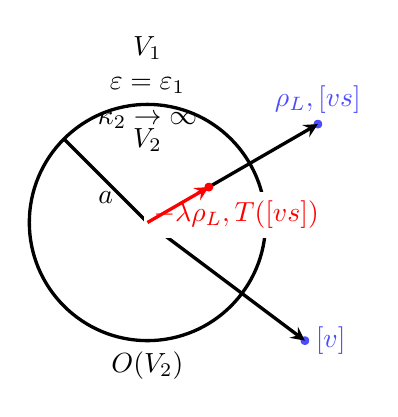
\begin{tikzpicture}[line width = 1.2pt, line join=round,>=stealth]
        \filldraw [color=blue!70] (30:2.5) circle (1pt) node[above] {$\rho_L, \Ortsr[vs]$}; 
        \filldraw [color=blue!70] (2,-1.5) circle (1pt) node[right] {$\Ortsr[v]$}; 
        \draw [-stealth] (0,0) -- (30:2.5); 
        \draw [-stealth] (0,0) -- (2,-1.5); 
        \draw (0,0) circle (1.5);
        \draw (0,0) -- (135:1.5);
        \draw (135:0.75 ) node[below] {$a$};
        
        \draw (0,-1.5) node [below] {$O(V_2)$};
        \draw(0,1.05) node {$V_2$};
        \draw(0,1.3) node{$\kappa_2 \to \infty$};
        \draw(0,2.0) node[align=center] {$V_1$\\$\varepsilon=\varepsilon_1$}; 
       \draw [color=red] (20:1.2) node[below, fill=white] {$-\lambda \rho_L, T(\Ortsr[vs])$}; 

       \draw [-stealth,color=red] (0,0) -- (30:0.9); 
       \filldraw [color=red] (30:0.9) circle (1pt);
      \end{tikzpicture}
      \end{column}
      \begin{column}{.7\textwidth}
        \begin{itemize}[<+->]
        \item Versuche wieder die \alert{Kelvin-Transformation}:
          \begin{equation*}
            T(\Ortsr[vs]) = \frac{a^2}{\left| \Ortsr[vs]\right|^2} \Ortsr[vs] = \frac{a^2}{(\rho^\prime)^2} \Ortsr[vs] 
          \end{equation*}
        \item Für das Potential gilt dann ($\lambda$ noch unbekannt)
          \begin{align*}
            \SkalarPot(a\vu{\rho}) & = -\frac{1}{2\pi\varepsilon_1}  \rho_L\left[\ln\left(\frac{\rho - a}{\rho_B} \right) -\lambda \ln\left(\frac{a - T(a\vu{\rho})}{\rho_B} \right)  \right] \stackrel{!}{=} 0 \\
            & \ln\left(\rho - a \right) -\lambda \ln(a - T(a\vu{\rho})) \stackrel{!}{=} 0 \\
            & \ln\left(\rho - a \right) -\lambda \ln(a - \frac{a^2}{\rho^2}\rho)) \stackrel{!}{=} 0 \\
            & \rho - a \stackrel{!}{=}  \left( a - \frac{a^2}{\rho}\right)^\lambda 
            \end{align*}
        \item Es gibt kein $\lambda$, das $\SkalarPot = 0$ auf der Oberfläche erzeugt.
          \end{itemize}
        \end{column}
      \end{columns}

    
    \end{frame}
  
    \begin{frame}
\frametitle{Linienladung vor Zylinder: $\lambda(\Ortsr[v])=1$}
\begin{itemize}[<+->]
\item Es gibt kein $\lambda$, das zusammen mit der Kelvin-Transformation das gewünschte Potential auf der Oberfläche des Zylinders erzeugt.
\item Trotzdem den Weg weiter beschreiten: setze $\lambda(\Ortsr[v])=1$
\item Wir hatten bereits:
  \begin{equation*}
    \left| T(\Ortsr[v]) - \Ortsr[vs]  \right| = \frac{\left| \Ortsr[vs]\right|}{\left| \Ortsr[v]\right|} \left| \Ortsr[v]   - T(\Ortsr[vs]) \right|
  \end{equation*}
\item Damit:
  \begin{align*}
    G_2(\Ortsr[v], T(\Ortsr[vs])) & = -\frac{1}{2\pi\varepsilon_1} \ln\left(\frac{\left|\Ortsr[v] - T(\Ortsr[vs])\right|  }{\rho_B} \right)  = -\frac{1}{2\pi\varepsilon_1} \ln\left(\frac{\left|T(\Ortsr[v]) - \Ortsr[vs]\right|  \left| \Ortsr[v]\right| }{\rho_B \left| \Ortsr[vs]\right|} \right) \\
                                            &= -\frac{1}{2\pi\varepsilon_1} \left[ \ln\left(\frac{\left|T(\Ortsr[v]) - \Ortsr[vs]\right| }{\rho_B } \right) + \ln\left(\frac{ \left| \Ortsr[v]\right| }{\rho_B } \right) - \ln\left(\frac{ \left| \Ortsr[vs]\right| }{\rho_B } \right)  \right]\\
    &= G_2(T(\Ortsr[v]), \Ortsr[vs]) + G_2(\Ortsr[v], \vec{0}) - G_2(0, \Ortsr[vs])    
  \end{align*}
\item Damit ist das Potential
  \begin{align*}
    \SkalarPot(\Ortsr[v]) & = \rho_L G_2(\Ortsr[v], \Ortsr[vs]) -\rho_L G_2(\Ortsr[v], T(\Ortsr[vs])) \\
    &= \rho_L \left[ G_2(\Ortsr[v], \Ortsr[vs]) - G_2(T(\Ortsr[v]), \Ortsr[vs]) - G_2(\Ortsr[v], \vec{0}) + G_2(0, \Ortsr[vs])\right]
    \end{align*}
  \end{itemize}
      \end{frame}

    \begin{frame}
\frametitle{Linienladung vor Zylinder: $\SkalarPot$ auf der Oberfläche}
\begin{itemize}[<+->]
\item Wir hatten das Potential berechnet:
  \begin{equation*}
    \SkalarPot(\Ortsr[v]) = \rho_L \left[ G_2(\Ortsr[v], \Ortsr[vs]) - G_2(T(\Ortsr[v]), \Ortsr[vs]) - G_2(\Ortsr[v], \vec{0}) + G_2(0, \Ortsr[vs])\right]
  \end{equation*}
\item Wegen $T(\Ortsr[v])=\Ortsr[v]$ für $\Ortsr[v] =a\vu{\rho} $ kompensieren sich die ersten beiden Terme auf der Oberfläche:
  \begin{equation*}
    \left.\SkalarPot(\Ortsr[v])\right|_{\Ortsr[v] =a\vu{\rho}} = \rho_L \left[ - G_2(a\vu{\rho}, \vec{0}) + G_2(0, \Ortsr[vs])\right] = \frac{\rho_L}{2\pi\varepsilon_1} \ln\left(\frac{a}{\abs{\Ortsr[vs]}} \right) 
  \end{equation*}
\item Vergleich mit Potential einer Linienladung auf der $z$-Achse:
  \begin{equation*}
      \SkalarPot(\Ortsr[v]) = -\frac{\rho_L}{2\pi\varepsilon_1} \ln\left(\frac{\rho}{\rho_B} \right) \rightarrow \left.\SkalarPot(\Ortsr[v])\right|_{\Ortsr[v] =a\vu{\rho}} = -\frac{\rho_L}{2\pi\varepsilon_1} \ln\left(\frac{a}{\rho_B} \right)
    \end{equation*}
  \item Offenbar lässt sich $\SkalarPot =0$ auf der Zylinderoberfläche durch eine zusätzliche Linenladung auf der $z$-Achse erreichen. Mit diesem Zusatz funktioniert hier also die Kelvin-Transformation mit $\lambda = 1$. $\to$ \alert{Problemangepasste Greensche-Funktion gefunden:}
    \begin{equation*}
      G^\star (\Ortsr[v], \Ortsr[vs]) = G_2(\Ortsr[v], \Ortsr[vs]) - G_2(\Ortsr[v], \frac{a^2}{(\rho^\prime)^2}\Ortsr[vs] )+ \left.G_2(\Ortsr[v], \vec{0})\right|_{\rho_B = \abs{\Ortsr[vs]}}
      \end{equation*}
  \end{itemize}
      \end{frame}



      
\input{finalframe.inc}
\end{document}